\section[Cote 76 : l'ordre des sommets ; drapeaux de type H, le lemme de surjectivité]{Cote 76 : l'ordre des sommets ; drapeaux de type $H$, le lemme de surjectivité\protect\verifie{Folder76}}\label{sec:76}

La cote 76, \emph{n-cartes cellulaires : notes manuscrites (s.d.)}, soixante-deux pages que l'inventaire date \q{[vers 1977]}, cherche une description combinatoire des complexes cellulaires et des cartes de dimension~$n$. Les pages~20 à~24 relient les ensembles semi-simpliciaux aux ensembles ordonnés munis d'un ordre sur les sommets ; la relation lue sur les arêtes, $x \prec y$, doit être transitive. La page~26 donne un second exemple (\q{Ex 2}) : un groupe $G$, des éléments $\sigma_0, \ldots, \sigma_n$ tels que $\sigma_i$ et $\sigma_j$ commutent pour $j \geq i + 2$, le sous-groupe $N_H$ engendré par les $\sigma_i$, $i \notin H$, un $G$-ensemble $X$ et ses \q{drapeaux de type $H$}, $D(H) = X/N_H$ (\lot{76}{2}{26}). La page~27 pose $x_i \prec y_j$ si $i < j$ et si $x_i$, $y_j$ ont un majorant commun, ramène la transitivité à la surjectivité de $D(\{i, j, k\}) \to D(\{i, j\}) \times_{D(\{j\})} D(\{j, k\})$ et énonce un lemme plus général, sous l'hypothèse \q{$H \cap H'$ \ldots{} segment final de l'ens tot.\ ordonné $H$, un segment initial de l'ens tot ordonné $H'$} (\lot{76}{2}{27}). La page~28 le démontre par la décomposition $G_{K \cup K'} \subset G_{K_0} \cdot G_{K'_0}$, et une note oblique dans la marge gauche dit n'avoir utilisé que \q{a) le dernier él.\ de $H$ est dans $H'$ ; b) $H \cap H'$ est un segment initial de $H'$} (\lot{76}{2}{28}). La lecture énonce le lemme sous ces deux hypothèses.

\noindent\emph{Conventions.} On note $\Delta_n = \{0, \ldots, n\}$, $G_K$ le sous-groupe de $G$ engendré par les $\sigma_i$, $i \in K$, pour $K \subset \Delta_n$, et $N_H = G_{\Delta_n \smallsetminus H}$. Pour $H \subset H'$, on a $N_{H'} \subset N_H$, d'où la restriction $D(H') \to D(H)$, $N_{H'}x \mapsto N_Hx$ ; elle est transitive. Aucune autre hypothèse n'est faite sur les $\sigma_i$ : ce ne sont pas nécessairement des involutions.

\begin{lemme}\label{lem:76-produit}
Soient $K, K' \subset \Delta_n$ et $i \in \Delta_n \smallsetminus (K \cup K')$ tels que tout $j \in K \cup K'$ avec $j < i$ soit dans $K'$ et tout $j \in K \cup K'$ avec $j > i$ soit dans $K$. Alors tout élément de $G_{K \cup K'}$ s'écrit $k'k$ avec $k' \in G_{K'}$ et $k \in G_K$.
\end{lemme}

\begin{proof}
Soient $A = G_{K'_0}$ et $B = G_{K_0}$, où $K'_0 = \{j \in K \cup K' : j < i\}$ et $K_0 = \{j \in K \cup K' : j > i\}$. Par hypothèse $A \subset G_{K'}$ et $B \subset G_K$. Un indice de $K'_0$ et un indice de $K_0$ diffèrent d'au moins~$2$, donc leurs générateurs commutent ; tout générateur de $B$ est alors dans le centralisateur de $A$, puis $B$ tout entier, et tout élément de $A$ commute à tout élément de $B$. L'ensemble $AB$ contient donc $1$, les générateurs $\sigma_j$, $j \in K \cup K'$ (qui sont dans $K'_0$ ou $K_0$ puisque $i \notin K \cup K'$), et il est stable par produit, $(ab)(a'b') = (aa')(bb')$, et par inverse, $(ab)^{-1} = a^{-1}b^{-1}$. Il contient le sous-groupe $G_{K \cup K'}$ qu'ils engendrent.
\end{proof}

\begin{theoreme}[Grothendieck, pages 27 et 28, lemme\piste{76-flag-presheaf-gset-lemma}]\label{thm:76-lemme}
Soient $G$ un groupe, $\sigma_0, \ldots, \sigma_n \in G$ tels que $\sigma_i$ et $\sigma_j$ commutent pour $j \geq i + 2$, et $X$ un $G$-ensemble. Soient $H, H' \subset \Delta_n$ tels que le plus grand élément de $H$ soit dans $H'$ et que $H \cap H'$ soit un segment initial de $H'$. Alors l'application
\[ D(H \cup H') \longrightarrow D(H) \times_{D(H \cap H')} D(H') \]
est surjective : deux drapeaux de types $H$ et $H'$ de même restriction à $H \cap H'$ sont les restrictions d'un même drapeau de type $H \cup H'$.
\end{theoreme}

\begin{proof}
Soient $a = N_Hx$ et $b = N_{H'}y$ de même image dans $D(H \cap H')$ : il existe $g \in N_{H \cap H'}$ avec $gy = x$. Posons $K = \Delta_n \smallsetminus H$ et $K' = \Delta_n \smallsetminus H'$, de sorte que $N_{H \cap H'} = G_{K \cup K'}$, et soit $i$ le plus grand élément de $H$. Il est dans $H \cap H'$, donc hors de $K \cup K'$. Un $j > i$ n'est pas dans $H$, donc est dans $K$. Un $j < i$ de $K \cup K'$ n'est pas dans $H'$ : sinon, $j \leq i$ avec $i \in H \cap H'$ et le segment initial le mettraient dans $H$, donc dans $H \cap H'$, ce qui contredit $j \in K \cup K'$. Le lemme~\ref{lem:76-produit} écrit $g^{-1} = k'k$ avec $k' \in N_{H'}$ et $k \in N_H$. Le drapeau $c$, classe de $kx$ dans $D(H \cup H')$, a pour image $N_Hkx = N_Hx = a$ dans $D(H)$, et, puisque $y = g^{-1}x = k'(kx)$, pour image $N_{H'}kx = N_{H'}y = b$ dans $D(H')$.
\end{proof}

\begin{corollaire}[page 27]\label{cor:76-transitif}
Pour $x \in D(\{i\})$ et $y \in D(\{j\})$, posons $x \prec y$ si $i < j$ et si $x$ et $y$ sont les restrictions d'un même drapeau d'un type $H \supset \{i, j\}$. Cette relation est transitive, pour tout $G$-ensemble $X$. Un majorant commun peut toujours être pris dans $D(\{i, j\})$, les sommets $i < j$ d'un même drapeau vérifient $\prec$, et $x \prec y$ n'a jamais lieu pour $x$ et $y$ de même type.
\end{corollaire}

\begin{proof}
La restriction d'un majorant de type $H$ à $\{i, j\}$ est un majorant de type $\{i, j\}$. Soient $i < j < k$, $x \prec y$ par $u \in D(\{i, j\})$ et $y \prec w$ par $v \in D(\{j, k\})$. On a $\{i, j\} \cap \{j, k\} = \{j\}$, qui est le plus grand élément de $\{i, j\}$ et un segment initial de $\{j, k\}$. Les restrictions de $u$ et $v$ à $\{j\}$ valent $y$, et le théorème~\ref{thm:76-lemme} donne $c \in D(\{i, j, k\})$ qui restreint à $u$ et à $v$, donc à $x$ et à $w$ : sa restriction à $\{i, k\}$ est un majorant commun de $x$ et $w$, et $i < k$.
\end{proof}

\begin{remarque}
Le lemme tient tel que la lecture l'énonce, sous les deux hypothèses de la note marginale, plus faibles que celles de l'énoncé de la page~27 : la non-vacuité de $H \cap H'$ découle de a), et le segment final de $H$ ne sert pas. La démonstration est celle de la page~28 ; la page écrit $G_{K \cup K'} = G_K \cdot G_{K'}$, le fichier en démontre l'inclusion sous la forme $G_{K'} \cdot G_K$, la seule dont la démonstration se sert. Les $\sigma_i$ ne sont pas supposés d'ordre~$2$, et le groupe, l'ensemble $X$ et l'action sont quelconques : la lecture le dit, et la page n'utilise en effet que la commutation des $\sigma_i$ éloignés. Le fichier formalise l'ordre des sommets sur $D_0 = \coprod_i D(\{i\})$ et sa transitivité, mais pas l'ensemble semi-simplicial qui en résulte. La piste demande si cette surjectivité, pour des $G$-ensembles quelconques, figure dans la théorie des géométries de classes de Tits ou des systèmes de chambres.
\end{remarque}

\paragraph{L'ordre des sommets (pages 20 à 24).} Un ensemble semi-simplicial $D$ satisfait (1) si les faces d'un simplexe sont deux à deux distinctes ; $D_* = \coprod D_m$, ordonné par \q{est face de}, satisfait alors (a). Sur $D_0$, $x \prec y$ s'il existe une arête de $x$ à $y$ ; (2 bis) demande que deux arêtes composables bordent un $2$-simplexe. La proposition des pages~23 et~24 met en correspondance les ensembles semi-simpliciaux satisfaisant (1) et \q{(2)}, chiffre incertain que la lecture lit comme la transitivité (2°), et les ensembles ordonnés satisfaisant (a) munis d'un ordre sur $D_0$ satisfaisant (b) et (c) (\lot{76}{1}{22}, \lot{76}{1}{24}).

\begin{theoreme}[D'après les pages 22 à 24, avec (2°)\piste{76-semisimplicial-vertex-order}]
Soit $D$ un ensemble semi-simplicial satisfaisant (1). Alors $D_*$ satisfait (a), les ordres de ses simplexes sont compatibles, et leur relation d'arête est $\prec$ ; la relation $\prec$ est transitive si et seulement si ces ordres sont tous induits par un même ordre sur $D_0$ satisfaisant (b) et (c), et cet ordre est alors $\prec$. Sur tout ensemble ordonné satisfaisant (a), les ordres sur $D_0$ satisfaisant (b) et (c) correspondent bijectivement, par restriction et par la relation d'arête, aux familles d'ordres totaux compatibles sur les simplexes dont la relation d'arête est transitive. Enfin (2 bis) entraîne (2°), et le bord d'un triangle satisfait (1) et (2°) sans satisfaire (2 bis).
\end{theoreme}

La figure~\ref{fig:76-ordres} donne trois cas, une flèche de $x$ vers $y$ figurant une arête de $x$ à $y$, donc $x \prec y$. Dans le premier, deux triangles pleins partagent une arête, et les ordres de leurs sommets sont induits par $v_0 < v_1 < v_2 < v_3$. Dans le deuxième, trois arêtes tournent : (1) tient, mais $v_0 \prec v_1 \prec v_2$ sans $v_0 \prec v_2$, et aucun ordre sur $D_0$ n'induit les ordres des arêtes. Le troisième est le bord d'un triangle orienté sans cycle.

\begin{figure}[htbp]
\centering
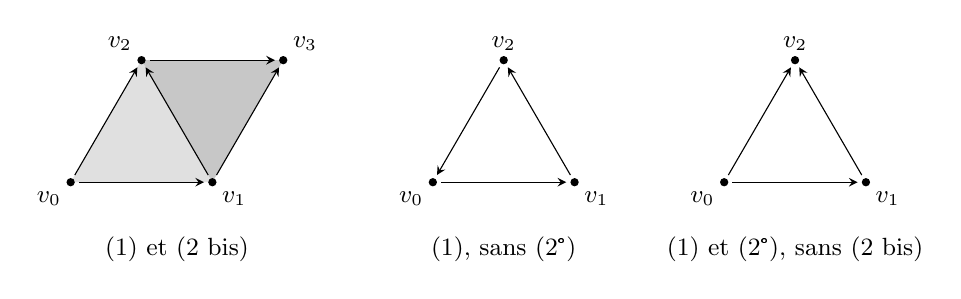
\begin{tikzpicture}[x=1cm, y=1cm, >=stealth, every node/.style={font=\small}]
\tikzset{ar/.style={->, shorten >=3pt, shorten <=3pt}}
\begin{scope}
\coordinate (v0) at (0,0); \coordinate (v1) at (1.8,0); \coordinate (v2) at (0.9,1.55); \coordinate (v3) at (2.7,1.55);
\fill[black!12] (v0)--(v1)--(v2)--cycle; \fill[black!22] (v1)--(v3)--(v2)--cycle;
\foreach \a/\b in {0/1,0/2,1/2,1/3,2/3} \draw[ar] (v\a)--(v\b);
\foreach \k in {0,...,3} \fill (v\k) circle (1.5pt);
\node[below left] at (v0) {$v_0$}; \node[below right] at (v1) {$v_1$}; \node[above left] at (v2) {$v_2$}; \node[above right] at (v3) {$v_3$};
\node at (1.35,-0.85) {(1) et (2 bis)};
\end{scope}
\begin{scope}[xshift=4.6cm]
\coordinate (v0) at (0,0); \coordinate (v1) at (1.8,0); \coordinate (v2) at (0.9,1.55);
\draw[ar] (v0)--(v1); \draw[ar] (v1)--(v2); \draw[ar] (v2)--(v0);
\foreach \k in {0,...,2} \fill (v\k) circle (1.5pt);
\node[below left] at (v0) {$v_0$}; \node[below right] at (v1) {$v_1$}; \node[above] at (v2) {$v_2$};
\node at (0.9,-0.85) {(1), sans (2°)};
\end{scope}
\begin{scope}[xshift=8.3cm]
\coordinate (v0) at (0,0); \coordinate (v1) at (1.8,0); \coordinate (v2) at (0.9,1.55);
\draw[ar] (v0)--(v1); \draw[ar] (v1)--(v2); \draw[ar] (v0)--(v2);
\foreach \k in {0,...,2} \fill (v\k) circle (1.5pt);
\node[below left] at (v0) {$v_0$}; \node[below right] at (v1) {$v_1$}; \node[above] at (v2) {$v_2$};
\node at (0.9,-0.85) {(1) et (2°), sans (2 bis)};
\end{scope}
\end{tikzpicture}
\caption{L'ordre des sommets. À gauche, deux $2$-simplexes (en gris) d'arête commune $v_1v_2$ : la relation d'arête est l'ordre $v_0 < v_1 < v_2 < v_3$, qui induit celui de chaque simplexe. Au milieu, trois arêtes en cycle, sans $2$-simplexe : $\prec$ n'est pas transitive. À droite, le bord du triangle : $\prec$ est l'ordre $v_0 < v_1 < v_2$, mais les arêtes composables $v_0v_1$ et $v_1v_2$ ne bordent aucun $2$-simplexe.}
\label{fig:76-ordres}
\end{figure}

{\sloppy \noindent L'énoncé tient avec (2°), comme la lecture le lit : voir \texttt{trans\_iff\_vertexOrder}, \texttt{vertexOrder\_unique}, \texttt{vertexOrderEquiv}, \texttt{isFlagGeom}, \texttt{trans\_of\_hornFill} et \texttt{triangleBoundary\_not\_hornFill} dans \href{\leanblob/Folder76.lean}{\texttt{Folder76.lean}}. Du côté des ensembles ordonnés, la correspondance n'utilise de (a) que l'existence, sous un simplexe, de l'arête qui joint deux de ses sommets. Le retour des ordres compatibles à l'ensemble semi-simplicial (pages~17 et~18) n'est pas refait ici : c'est le cas $M = \Delta_{\mathrm{inj}}$ de l'équivalence de la cote~104 (§\,\ref{sec:104}).\par}

Ne sont pas démontrés ici : la condition (a) pour $D_* = \coprod_H D(H)$ et l'ensemble semi-simplicial qu'elle définit, avec $D_m = \coprod_{\operatorname{card} H = m+1} X/N_H$ ; le programme de la page~29.
